\documentclass[output=paper]{langsci/langscibook} 
\ChapterDOI{10.5281/zenodo.4545033}
\author{Shaimaa Marzouk\affiliation{Johannes Gutenberg University Mainz}}


\title[German light verb construction in the course of the development of MT]
      {German light verb construction in the course of the development of machine translation}

\abstract{The German light verb construction \textsc{(lvc)} is commonly used despite its relative complexity. Different writing guidelines recommend avoiding \textsc{lvc}s and replacing them with the base verb constructions (\textsc{bvc}s). However, since not every \textsc{lvc} has an equivalent \textsc{bvc}, replacement is not always possible. The present study addresses two aspects: first, how the machine translation \textsc{(mt)} of \textsc{lvc} has evolved in light of recent progress in \textsc{mt} and the increasing dominance of neural machine translation \textsc{(nmt)}, and second, whether the use of \textsc{bvc}s improves \textsc{mt} output compared to \textsc{lvc}s. The analysis of the \textsc{mt} output of both scenarios, \textsc{lvc} and \textsc{bvc}, is performed for different \textsc{mt} approaches in terms of number and types of \textsc{mt} errors, style and content quality ratings, and scores from two automatic evaluation metrics (\textsc{aem}s). For this, a mixed-methods triangulation approach that includes error annotation, human evaluation, and automatic evaluation was applied and five \textsc{mt} systems were examined: a rule-based system \textsc{(rbmt)}, a statistical system \textsc{(smt)}, two differently constructed hybrid systems \textsc{(hmt)}, and a neural system \textsc{(nmt)}. The study is conducted for the language pair German-to-English in the technical domain. The results show that systems that employ earlier \textsc{mt} approaches \textsc{(rbmt, smt, hmt)} benefited from replacing the \textsc{lvc} with the corresponding \textsc{bvc} as their output was improved (i.e., \textsc{mt} errors were reduced; quality and \textsc{aem}s scores were increased). On the contrary, the \textsc{nmt} system was able to produce \textsc{mt} with minimal number of errors both for \textsc{lvc}s and \textsc{bvc}s and recorded the highest quality levels in both scenarios among the analyzed \textsc{mt} systems.}

\begin{document}
\SetupAffiliations{mark style=none}
\maketitle

\section{Introduction}\label{marzouk:introduction}

The German term \textit{Funktionsverbgefüge} was coined by \citet[26]{vonPolenz1963}; the English counterpart, \textit{function verb constructions} or \textit{light verb constructions}, hereafter \textsc{lvc}s, goes back to the linguist \citet[117]{Jespersen1942}. With this, Jespersen (ibid.) distinguishes between a light verb and a heavy verb (a.k.a. \textit{full verb}, a verb that emphasizes the full meaning). Some examples of \textsc{lvc}s are: 
\textit{eine Frage stellen} (`to pose a question'), where \textit{stellen} is a light verb, as opposed to \textit{fragen} (`to ask'), which acts as a full verb; \textit{eine Handlung ausführen} (`to perform an action') to replace the full verb \textit{handeln} (`to act'); \textit{etw. zu Papier bringen} (`to put sth. on paper') instead of \textit{schreiben} (`to write'), and \textit{eine Entscheidung treffen} (`to make a decision') instead of \textit{sich entscheiden} (`to decide'). 

As illustrated by these examples, an \textsc{lvc} is simply a combination of a verb and a noun that can only be correctly understood with both components. Strictly speaking, it is a complex predicate that consists of a semantically light verb and a deverbal noun \citep[117]{Jespersen1964}. The verb in the \textsc{lvc} acts merely as a functional element, letting the noun represent the main predicate \citep{Grimshaw1988}. The \textsc{lvc} is not just found in German, but in many other languages as well. In English, \textit{make a decision} is sometimes used instead of \textit{decide}. Similarly, in Arabic, one might say \textit{yakhudh qraraan} (`make a decision') or  \textit{yuqrĩr} (`decide').\footnote{The Arabic examples were transliterated by \url{https://de.glosbe.com/transliteration/Arabic-Latin}.} Both variants also exist in Spanish \textit{tomar una decisión} (`make a decision') and \textit{decidir} (`decide').

The present study focuses on German \textsc{lvc}s that can take on one of the following forms: a verb plus a noun in the accusative case (e.g., \textit{eine Handlung ausführen}) or a verb plus a prepositional phrase (e.g., \textit{zu Papier bringen}). German \textsc{lvc}s are used predominantly in technical, scientific, legal, and official texts \citep[38f.]{Bruker2013}, but despite their widespread use, they are criticized both in linguistics and translation. In linguistics, they are seen as a sign of “Umschreibungssucht” (addiction to reformulating) and “Verbaphobie” (verbaphobia) \citep[9f.]{Daniels1963} and have been described as “unnecessarily complicated” and “inelegant” \citep{Storrer2006a}. Because of the relative complexity of \textsc{lvc}s, several Controlled Language varieties and writing guidelines prompt writers to avoid them: (1) The rule “Avoid light verb constructions” is found in Leichte Sprache (Easy German Language), which is increasingly being applied to simplify legal, political, and administrative texts for people with low language skills or cognitive limitations \citep{Hansen-Schirra2018}. Here, the rule is included to reduce sentence complexity \citep{ubhd-67957969}. (2) The rule is also applied in Controlled Languages used in technical documentation in order to keep sentences more concrete and direct \citep[107]{GesellschaftfurTechnischeKommunikation2013}. (3) The same rule is present in the guidelines from the weekly German magazine \textit{Die Zeit} entitled \textit{Recommendations for prospective journalists}, which advise journalists to use full verbs instead of \textsc{lvc}s, as full verbs are usually clearer and more efficient \citep{Zeit2007}.

However, despite their structural complexity, \textsc{lvc}s are widely used. This is partially due to the fact that some \textsc{lvc}s completely lack any equivalent, e.g., \textit{in Ordnung halten} (`to keep in order'). Other \textsc{lvc}s have a more nuanced meaning that can be difficult to express using the base verb construction, hereafter \textsc{bvc}. One example of this kind of \textsc{lvc} is \textit{eine Maschine in Betrieb setzen} (`to put a machine into operation'); this is a process that usually includes several different procedures depending on the complexity of the machine and is therefore much more than simply (p. 107) \textit{eine Maschine einschalten} (`to turn on a machine') \citep{ubhd-67954849}. Concretely, the \textsc{lvc}s can influence meaning in four ways, which are known as “action types” \citep*[704]{Zifonun1997}:


\begin{description}
\item [Causative:] emphasize the initiator of an action, e.g., \textit{der Starter setzt den Motor in Gang} (`the starter sets the engine in motion').

\item [Inchoative:] mark the beginning of an action, e.g., \textit{endlich geht das Buch in Druck} (`finally, the book goes to press').

\item [Durative:] emphasize the duration of an action, e.g., \textit{ein neues Modell ist bereits in Arbeit} (`a new model is already in production').

\item [Passive:] form a distinct passive meaning variation, e.g., \textit{die neue Methode findet Anwendung bei dem Versiegelungsprozess} (`the new method is applied in the sealing process').
\end{description}

\section{Machine translation of \textsc{lvc}s}
As discussed, the usage of the \textsc{lvc}s can be indispensable in conveying a distinct nuance of meaning or because there is no \textsc{bvc} equivalent. Despite the existence of \textsc{lvc}s in several languages, there are a number of difficulties in \textsc{mt} of \textsc{lvc}s. \citet{Heine2017} describes \textsc{lvc}s as “a typical example of phenomena that are neither explainable with (exclusively) grammatical rules nor lexical units” and how the sentence syntax as well as the lexical components of the \textsc{mt} system are decisive for an error-free \textsc{mt} output. Therefore, depending on the complexity of the sentence syntax and the \textsc{mt} system approach as well as the system capacity, the primary challenge of translating an \textsc{lvc} is that the parser must first identify it as such. The system needs to be able to distinguish between \textit{stellen} as a full verb, as in \textit{etwas auf den Tisch stellen} (`to put something on the table') as opposed to \textit{stellen} as a light verb in \textit{etwas zur Verfügung stellen} (`to make something available'), \textit{eine Frage stellen} (`to ask a question'), or \textit{etwas in Rechnung stellen} (`to invoice something').


After identifying the \textsc{lvc} in the source language, a transfer problem between the source and target language may appear. Depending on the language pair, the \textsc{lvc} might be (best) translated using an equivalent \textsc{lvc}, a different function verb, a \textsc{bvc}, or a completely different construction \citep[96]{Bruker2013}, e.g., translating \textit{zur Verfügung stehen} as `are available'. In addition, a syntactic translation problem may arise while translating \textsc{lvc}s with prepositional phrases that have no articles or with a preposition that can require different cases, such as \textit{in}, \textit{an}, \textit{auf}, or \textit{unter}, e.g., \textit{in Betrieb nehmen} (accusative) vs. \textit{in Betrieb bleiben} (dative) or \textit{in Verhandlungen treten} (accusative) vs. \textit{in Verhandlungen stehen} (dative). Such cases cannot be strictly morphologically differentiated. The correct case for the output of the syntax information for the nominal phrase in the \textsc{lvc} can probably only be determined by using appropriate lexicon entries for the function verb, as the verb selects the case of the prepositional phrase. (ibid.: 75) Another potential problem can be encountered on a morpho-syntactic level in processing \textsc{lvc}s that include compounds, e.g., \textit{Verstellung vornehmen} in \textit{Höhenverstellung vornehmen} or \textit{Behandlung durchführen} in \textit{Fleckenbehandlung durchführen}. In such cases, the \textsc{lvc} with the compound must first be morpho-syntactically analyzed and broken down into its component parts \citep{Winhart2005}. For this, an exact semantic analysis of the compound is required for a correct processing of the \textsc{lvc} \citep[97]{Bruker2013}.


The difficulties in the \textsc{mt} of \textsc{lvc}s as well as their frequent use in the German language make its relevance for Natural Language Processing evident. Nonetheless, the \textsc{lvc} has not yet received the attention it needs in computational linguistics, particularly in \textsc{mt} research. There is a number of linguistic studies that closely investigate the linguistic differences between \textsc{lvc}s and \textsc{bvc}s on the basis of corpora \citep{Glatz2006,Storrer2007,Storrer2006a}. \citet{Storrer2006a} shows how the influence of both constructions goes beyond their different pragmatic and stylistic impacts. Others investigated the properties of multiword predicates and developed automatic methods for distinguishing among literal, metaphorical, and idiomatic multiword predicates \citep*{Fazly2005}. \citet{North2005} examined the productivity of \textsc{lvc}s that include predicative nouns and developed computational measures for quantifying the acceptability of \textsc{lvc}s. \citet{Kuhn1994} analyzed how the \textsc{hpsg}-based translation approach\footnote{\textsc{hpsg}: Head-driven Phrase Structure Grammar \citep{Pollard1994}
was considered the best available grammar formalism at that time.} handles \textsc{lvc}s. \citet{Marzouk2019} analyzed the impact of avoiding \textsc{lvc}s among other German Controlled Language rules on machine translatability across different \textsc{mt} approaches and found out that the \textsc{nmt} system delivers in comparison to \textsc{rbmt}, \textsc{smt} and hybrid \textsc{mt} systems mostly error-free output both before and after the application of the rules showing even a decrease in quality after applying the rules. Further studies on \textsc{mt} of German \textsc{lvc}s across different \textsc{mt} approaches including the \textsc{nmt} have not yet been conducted, to the best of my knowledge. In light of the proven linguistic differences between \textsc{lvc}s and \textsc{bvc}s \citep{Glatz2006,Storrer2007,Storrer2006a} and the success achieved by \textsc{nmt} in improving \textsc{mt} output compared to earlier approaches \citep{Bentivogli2016,Marzouk2019,Popovic2018,Toral2017,}, this study aims to track \textsc{mt}’s progress in translating \textsc{lvc}s.

The remainder of this paper is organized as follows: \sectref{marzouk:desofst} provides an overview of the empirical study including the dataset and the \textsc{mt} systems used. \sectref{marzouk:meth} outlines the methodology applied. Results are presented in \sectref{marzouk:res} followed by a discussion in \sectref{marzouk:dis}. Finally, \sectref{marzouk:con} provides the conclusion, mentions the limitations of the study, and gives an overview of future work.

\section{Description of study}\label{marzouk:desofst}


The study analyzes two aspects of \textsc{mt} with regard to \textsc{lvc}s: (1) to what degree different \textsc{mt} approaches are able to translate \textsc{lvc}s and (2) whether the use of \textsc{bvc}s improves the \textsc{mt} compared to using \textsc{lvc}s. In the analysis, \textsc{mt} outputs of \textsc{lvc}s and \textsc{bvc}s are contrasted across four \textsc{mt} approaches, and the impact of each construction is measured in terms of number and types of \textsc{mt} errors, style and content quality ratings, and \textsc{aem}s scores. The examined \textsc{mt} approaches are represented by five \textsc{mt} systems: Google Translate (an \textsc{nmt} system), Lucy \textsc{lt} \textsc{kwik} Translator (an \textsc{rbmt} system), \textsc{sdl} Free Translation (an \textsc{smt} system), and Bing by Microsoft and Systran (two differently constructed \textsc{hmt} systems).\footnote{The \textsc{mt} step was performed at the end of $2016$. At that time, Bing became an \textsc{hmt} system by adding language-specific rule components to its original \textsc{smt} system, and Systran was also developed from an \textsc{rbmt} system into a hybrid system.} The selection criteria of the systems were (1) to be an online freely available system, (2) to offer the language pair German-to-English, and (3) to cover different \textsc{mt} approaches.

For the analysis, a test suite was constructed that consists of 24 source sentences extracted from a corpus of German technical user manuals using the Controlled Language checker \textsc{clat} \citep{Rosener2010}.\footnote{ \textsc{clat} is one of the most well-known Controlled Language checkers in Germany developed by the society for the promotion of applied information sciences (\textsc{iai}) at Saarland University; see: \url{http://www.iai-sb.de/de/produkte/clat}.} The 24 analyzed \textsc{lvc}s were as follows: twelve accusative \textsc{lvc}s and twelve prepositional \textsc{lvc}s. After reformulating the sentences using the \textsc{bvc}s, both versions (\textsc{lvc}s and \textsc{bvc}s) were machine translated into English using the aforementioned five \textsc{mt} systems, resulting in a dataset of 240 \textsc{mt} sentences (24 source sentences $\times$ 2 versions $\times$ 5 systems). In the source sentences, company-specific and specialist terms were replaced with common terms (e.g. \textit{Gerät} instead of \textit{Feinstzerkleinerer}; \textit{Steckdose} instead of \textit{Schutzkontaktsteckdose}). This modification was necessary for two reasons: (1) the \textsc{mt} systems used in the study were not trained in advance with specific relevant corpora; (2) to avoid human evaluators investing too much time investigating the translation of these types of uncommon terms during the human evaluation. Source sentences that included more than two specific terms were excluded entirely from the analysis to avoid application of multiple changes to the original source sentences.


\section{Methodology}\label{marzouk:meth}

A mixed methods triangulation approach was applied that incorporates three evaluation methods: error annotation, human evaluation, and automatic evaluation. The analyses were conducted in a black box context, as the focus is on the comparison of the \textsc{mt} outputs of the \textsc{lvc} and \textsc{bvc} scenarios (and not on the internal processes of the systems). In the following, the analyses are demonstrated in detail.

\subsection{Error annotation}

The goal of the error annotation is to identify the \textsc{mt} errors in the use of \textsc{lvc}s (\textsc{lvc} scenario) and \textsc{bvc}s (\textsc{bvc} scenario) and compare them in terms of their number and type. The annotation was conducted by a qualified experienced German–English translator and checked by two professional German–English translators. Further, based on the existence or non-existence of \textsc{mt} errors, the data were divided into four groups, referred to as ``annotation groups''. These are: \textsc{ff} (for false-false): translation contains error(s) in both scenarios; \textsc{fr} (for false-right): translation contains error(s) only in the \textsc{lvc} scenario; \textsc{rf} (for right-false): translation contains error(s) only in the \textsc{bvc} scenario; \textsc{rr} (for right-right): no errors in either scenario. The error classification applied is mainly based on \citet{Vilar2006} and encompasses the error types shown in \tabref{marzouk:table1}.\footnote{As the analysis of the \textsc{lvc}s and \textsc{bvc}s was part of a large-scale study that aimed to examine different German Controlled Language rules, it was necessary to add two further relevant error types to \citet{Vilar2006}'s taxonomy (capitalization and consistency) and to exclude two error types in Vilar et al. (ibid.) that were irrelevant for the study (idioms and style).}


\begin{table}
\begin{tabularx}{\textwidth}{llQ}
\lsptoprule
% Error
Category  &
% Error
No. &
% Error
Type\\
\midrule
Orthography  &  \textsc{or}.\oldstylenums{01} & Punctuation error\\
             &  \textsc{or}.\oldstylenums{02}  &  Capitalization error\\
\midrule
Lexis  &     \textsc{lx}.\oldstylenums{03}   &   Omission\\
       &     \textsc{lx}.\oldstylenums{04} &   Addition\\
       &     \textsc{lx}.\oldstylenums{05} &   Untranslated\\
       &     \textsc{lx}.\oldstylenums{06} &  Consistency error (a word is repeated in the sentence  and translated differently each time)\\
\midrule
Grammar  &   \textsc{gr}.\oldstylenums{07}  &    Wrong word class\\
         &   \textsc{gr}.\oldstylenums{08}  &    Wrong verb tense / composition / person\\
         &   \textsc{gr}.\oldstylenums{09}  &    Wrong agreement gender / number / person\\
         &   \textsc{gr}.\oldstylenums{10}  &    Wrong word order\\
\midrule
Semantics & \textsc{sm}.\oldstylenums{11} & Confusion of sense (output translation is possible,  but not in the given context)\\
          & \textsc{sm}.\oldstylenums{12} &  Wrong choice (output translation is apparently wrong)\\\
          & \textsc{sm}.\oldstylenums{13} & Collocation error\\
\lspbottomrule
\end{tabularx}
\caption{Error classification applied in the annotation\label{marzouk:table1}}
\end{table}


The error taxonomy of \citet{Vilar2006} was used as a basis for the error annotation due to its explicity, clarity and appropriate degree of granularity. However, further more extensive taxonomies, such as the multidimensional quality metrics (\textsc{mqm}) framework can be also used for the analysis. This would be particularly useful in case of examining fine-grained or more specific types of errors.


\subsection{Human evaluation}\largerpage

The goal of the human evaluation is to compare the content and style quality of the \textsc{mt} in the \textsc{lvc} and \textsc{bvc} scenarios. Following the quality definition of \citet{Hutchins1992}, the \textit{content quality} is the extent to which the translation reflects the information in the source text accurately; and the extent to which the translation is easy to understand (ibid.). The \textit{style quality} is the extent to which the translation sounds natural and idiomatic in standard written English, is appropriate for the intention of its content (ibid.) as well as presented clearly in terms of orthography. The definition covers the orthography as an instrument for presenting the content in an adequate way that serves its intention. 

Based on these definitions, the content quality (\textsc{cq}) covers the criteria accuracy and clarity; the style quality (\textsc{sq}) encompasses the criteria idiomaticity, appropriateness to the content intention as well as correctness and clarity of the orthographic presentation. 

The human evaluation \figref{marzouk:fig1} consisted of
(1) evaluating the \textsc{sq} and \textsc{cq} of the \textsc{mt} (*) on two 5-point Likert scales;
(2) selecting the relevant quality criteria that justify the assigned quality scores: accuracy and clarity under the \textsc{cq}; idiomacy, appropriateness to the content intention as the content well as correctness and clarity of the orthographic presentation under the \textsc{sq};
(3) providing the word or part of the translation relevant to each chosen criterion; (4) where many modifications were necessary, the participant had to enter an alternative translation for the whole sentence.\largerpage[2]


\begin{figure}
	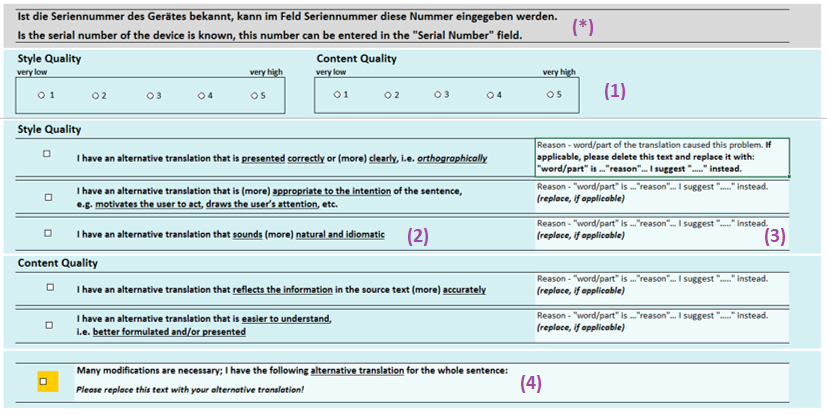
\includegraphics[width=\textwidth]{figures/figure1.png}
    \caption{Interface of the human evaluation}
    \label{marzouk:fig1}
\end{figure}


Concerning the participants, different studies recommend recruiting more\linebreak than 3--4 participants \citep{Fiederer2009}. In this study, five participants initially conducted the tests and the number of participants was successively increased until the accumulated average of the quality values stabilized. After the eighth participant, the accumulated quality averages hardly changed. Accordingly, the number of participants was not increased anymore. The participants are native English speakers and hold a bachelor’s degree in translation. In addition, all participants were students in the last or penultimate semester of the master’s degree program in translation. Participation was remunerated.

Regarding the test procedure, the analysis of the \textsc{lvc}s and \textsc{bvc}s was part of a large-scale study that aimed to examine different German Controlled Language rules \citep{Marzouk2019}. Within the scope of the study, each participant evaluated in total 1,100 \textsc{mt} sentences that were randomized and split into 44 tests (the analysis of the \textsc{lvc} vs. \textsc{bvc} was a subset of this dataset). Each participant had the opportunity to choose whether to rate one, two or three tests per day, depending on his or her availability. The basic requirement was to evaluate at least one test daily, thus avoiding interruptions that could possibly have a negative effect on the intra-rater agreement. In addition, the participants were asked to take a break between the tests. The 44 tests were sent in a different randomized order to the participants (e.g. the 1st participant received test 40, test 8, test 5 consecutively). A decreasing motivation over a 3--4 week evaluation period is unavoidable. Therefore, this randomization ensured that no particular sentences were evaluated by all participants at the end of the evaluation. The tester received the answered tests every day and checked them for completeness (i.e. all sentences were rated and commented on if necessary). In case of any missing data, the participant was asked to complete them, then he or she received the new tests for the next day.

\subsection{Automatic evaluation}\largerpage


The alternative translation obtained from the human evaluation acted as a reference translation for the automatic evaluation metrics (\textsc{aem}s) in order to compare their scores in the \textsc{lvc} and \textsc{bvc} scenarios. Two reference translations per sentence were randomly selected for the comparison. The study applied the evaluation metrics \textsc{ter}base and h\textsc{lepor}. The former is a basic edit distance metric that calculates the minimum number of edits needed to change the evaluated \textsc{mt} so that it exactly matches the reference translation and works without stemming, synonymy lookup and paraphrase support \citep{Snover2006,Gonzalez2014}. It was necessary to consider the use of synonyms as an edit, as the participants quite often recommended the use of a certain synonym while evaluating the translation accuracy. At the same time, h\textsc{lepor} was applied as one of the advanced metrics that has proven to have a state-of-the-art correlation with human evaluation compared with metrics like \textsc{bleu}, \textsc{ter}, and \textsc{meteor} among others \citep{Han2013}. The calculation model of h\textsc{lepor} is based on three factors: an enhanced length penalty, an $n$-gram position difference penalty and the harmonic mean of precision and recall (ibid.).


\section{Results}\label{marzouk:res}

\subsection{Analysis of the annotation groups (\textsc{ff}, \textsc{fr}, \textsc{rf}, \textsc{rr}) based on the error annotation}


Comparing the \textsc{lvc} and \textsc{bvc} scenarios (\figref{marzouk:fig2}) showed that 42\% of the sentences were translated correctly in both scenarios (group \textsc{rr}), while half of this percentage (21\%) was translated incorrectly in both scenarios (group \textsc{ff}). At the same time, 29\% of the sentences were translated incorrectly while using the \textsc{lvc}s and correctly after using the \textsc{bvc}s (group \textsc{fr}). On the other hand, 8\% were only translated incorrectly while using the \textsc{bvc}s (group \textsc{rf}).


\begin{figure}
% 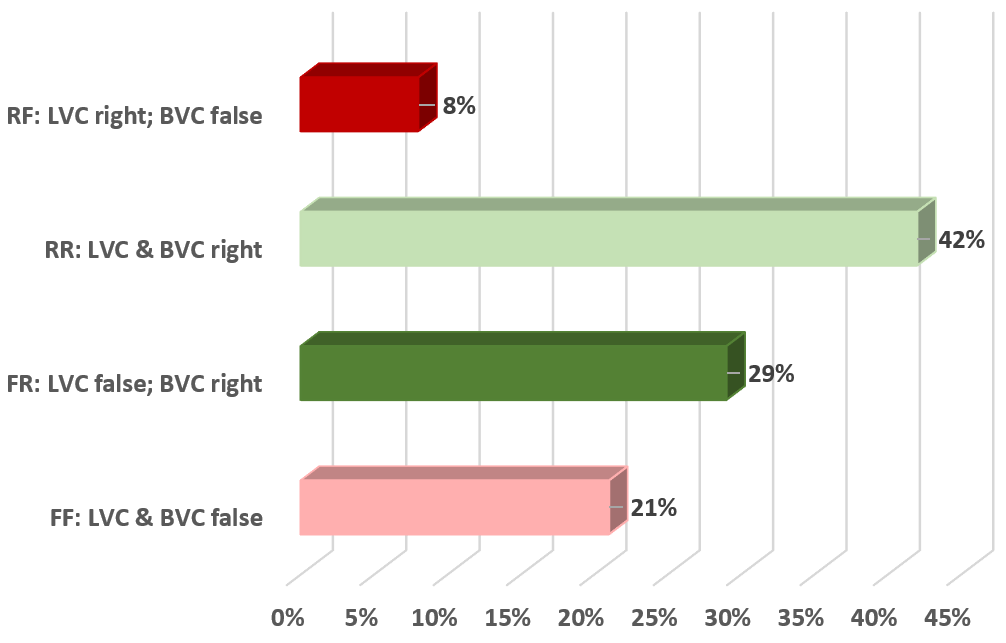
\includegraphics[scale=0.45]{figures/figure2.png}
    \begin{tikzpicture}
        \begin{axis}[
            xbar,
            xmin=0,
            axis lines*=left,
            width  = .7\textwidth,
            height = .3\textheight,
            xlabel={\%},
            symbolic y coords={%
                {{FF: LVC \& BVC false}},
                {{FR: LVC false, BVC right}},
                {{RR: LVC \& BVC right}},
                {{RF: LVC right, BVC false}}
            },
            ytick=data,
            tick label style={font=\footnotesize},
            nodes near coords,
            nodes near coords style={font=\footnotesize},
            nodes near coords align={horizontal},
            ]
            \addplot[black,fill=black] coordinates {
                (21,{{FF: LVC \& BVC false}})
                (29,{{FR: LVC false, BVC right}})
                (42,{{RR: LVC \& BVC right}})
                (8,{{RF: LVC right, BVC false}})
            };
        \end{axis}
    \end{tikzpicture}

\caption{Distribution of annotation groups for all the MT systems}
\label{marzouk:fig2}
\end{figure}



Based on the existence and non-existence of \textsc{mt} errors, the impact of using the \textsc{bvc} instead of the \textsc{lvc} on the \textsc{mt} output cannot be considered effectively positive. The only positive impact can be observed in the \textsc{fr} group (false in case of \textsc{lvc} -- right in case of \textsc{bvc}). This group amounts to 29\%. At the same time, the groups \textsc{rf} and \textsc{ff} together amount to 29\%: In \textsc{rf} (right in case of \textsc{lvc} -- false in case of \textsc{bvc}), there is a clear negative impact of using the \textsc{bvc} and in \textsc{ff} the usage of the \textsc{bvc} did not help produce an error-free \textsc{mt}.

Considering the groups \textsc{rr} and \textsc{ff}, since the translations were both in the \textsc{lvc} scenario and the \textsc{bvc} scenario correct (\textsc{rr} group) or incorrect (\textsc{ff} group), a positive impact of a certain scenario can only be justified if its quality values in these two groups were higher. In order to explore quality changes in each annotation group, the results of the error annotation and human evaluation were triangulated. The triangulated results showed no significant quality changes in the \textsc{rr} and \textsc{ff} groups. The only significant quality change was in a few cases of the group \textsc{fr}, indicating that getting an incorrect \textsc{mt} of the \textsc{lvc} and a correct \textsc{mt} of the \textsc{bvc} led to significantly higher quality in case of the \textsc{bvc}. 

\subsection{Analysis of the error types}
On the semantic level, the three semantic error types \textsc{sm}.\oldstylenums{11} confusion of sense, \textsc{sm}.\oldstylenums{12} wrong choice and \textsc{sm}.\oldstylenums{13} collocation error were affected in both scenarios. However, a significant change in the number of errors was only observed in error type \textsc{sm}.\oldstylenums{13} collocation error; this decreased significantly after replacing the \textsc{lvc} with a \textsc{bvc}. Furthermore, in few cases, the grammatical error types \textsc{gr}.\oldstylenums{08} wrong verb and \textsc{gr}.\oldstylenums{10} wrong word order and the lexical error type \textsc{lx}.\oldstylenums{04} addition were differently affected in both scenarios without showing a significant increase or decrease in a certain scenario. The remaining error types were not relevant.

\subsection{Analysis of the quality changes based on the human and automatic evaluations}
Although the analysis of the annotation groups did not reflect a substantial quality increase after using the \textsc{bvc} except for the aforementioned significant quality change in group \textsc{fr}, a significant increase in the \textsc{mt} quality in terms of style and content quality (\textsc{sq} and \textsc{cq}) as well as \textsc{aem}s scores was detected based on the human and automatic evaluations where the \textsc{bvc} was used.



Furthermore, the Spearman test was conducted to investigate the correlation between the difference in the overall quality\footnote{The overall quality is the mean of \textsc{sq} and \textsc{cq}, as analyzing the correlation here requires no distinction between the quality parameters.} and the differences in the \textsc{aem}s scores in both scenarios. The test showed a significant positive strong correlation ($\rho > 0.5, p < 0.001$). Accordingly, the quality changes detected in both analyses (human and automatic evaluation) were in line with each other.



\subsection{Comparison of the impact of replacing the \textsc{lvc} with the \textsc{bvc} at \textsc{mt} system level}
So far, the results show that the \textsc{mt} of \textsc{bvc}s had a significant higher quality in terms of human scores of the \textsc{sq} and \textsc{cq} as well as \textsc{aem}s scores. Subsequently, an analysis at \textsc{mt} system level was conducted in order to explore which \textsc{mt} systems exhibited these higher quality levels. The general positive impact of using \textsc{bvc}s instead of \textsc{lvc}s on the \textsc{mt} output at system level is shown in \figref{marzouk:fig3} and \figref{marzouk:fig4}.



\begin{figure}[p]
	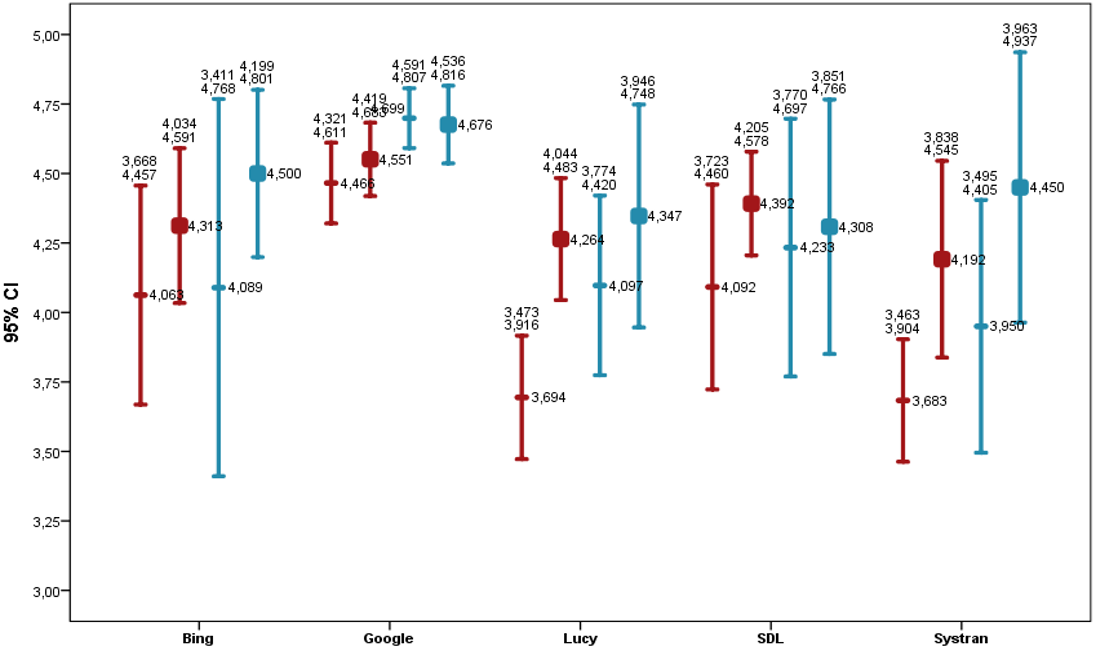
\includegraphics[width=\textwidth]{figures/figure3.png}
    \caption{Style and content quality in case of using \textsc{lvc}s as opposed to \textsc{lvc}s\label{marzouk:fig3}}
\end{figure}

\begin{figure}[p]
% 	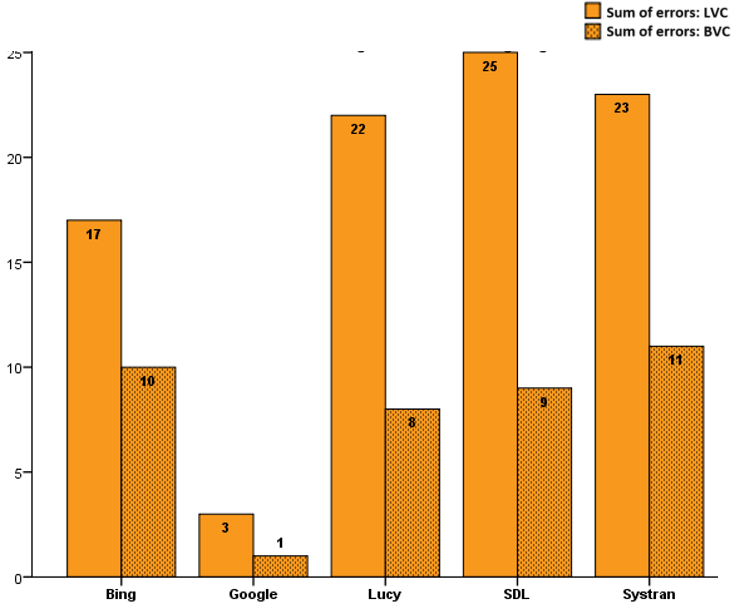
\includegraphics[width=\textwidth]{figures/figure4.png}

	  \begin{tikzpicture}
    \begin{axis}[
        axis lines*=left,
        width  = \textwidth,
        height = .3\textheight,
        nodes near coords,
        xtick=data,
        x tick label style={},
        ybar,
        bar width=.7cm,
        ymin=0,
        symbolic x coords={Bing,Google,Lucy, SDL, Systran},
        legend cell align=left,
        legend pos=north west,
        enlarge y limits = {upper, abs value=10}
        ]
        \addplot[black,fill=black] plot coordinates {
            (Bing,17)
            (Google,3)
            (Lucy,22)
            (SDL,25)
            (Systran,23)
        };
        \addplot[black!40,fill=black!40] plot coordinates {
            (Bing,10)
            (Google,1)
            (Lucy,8)
            (SDL,9)
            (Systran,11)
        };
        \legend{Sum of errors: LVC, Sum of errors: BVC}

    \end{axis}
  \end{tikzpicture}
    \caption{Number of \textsc{mt} errors in case of using 
\textsc{lvc}s as opposed to \textsc{bvc}s }
    \label{marzouk:fig4}
\end{figure}\pagebreak



For the \textsc{rbmt} system (Lucy) and one hybrid system (Systran), using the \textsc{bvc} was very advantageous in reducing the number of errors and increasing \textsc{sq} significantly. In the other hybrid system (Bing) and the \textsc{smt} system \textsc{(sdl)}, the number of errors decreased and the \textsc{sq} and \textsc{cq} increased after using the \textsc{bvc}; however, the changes were not significant. The \textsc{nmt} system (Google Translate) showed distinct results: the number of errors was minimal (three errors in the \textsc{lvc} scenario; one error in the \textsc{bvc} scenario). \textsc{gnmt} was able to translate 88\% of the sentences in both scenarios correctly, followed by Bing with 46\%, and recorded the highest \textsc{sq} and \textsc{cq} among all systems in both scenarios as well.



\subsection{Correlation between the error types and the quality values}\largerpage[2]
The earlier \textsc{mt} approaches showed the following significant strong correlations between a decreased number of errors of the different error types and increased quality values when using a \textsc{bvc}: In Lucy, the decrease in the semantic errors \textsc{sm}.\oldstylenums{11} confusion of sense and \textsc{sm}.\oldstylenums{12} wrong choice correlated with the increase in \textsc{sq} ($\rho = -0.521, p = 0.027$) and \textsc{cq} ($\rho = -0.537, p = 0.021$) respectively. In Bing, there was a correlation between the error type \textsc{lx}.\oldstylenums{03} omission and \textsc{cq} ($\rho = -0.565, p = 0.035$). In \textsc{sdl}, the correlation was observed between each of the error types \textsc{lx}.\oldstylenums{04} addition and \textsc{gr}.\oldstylenums{10} wrong word order and the \textsc{sq} (for \textsc{lx}.\oldstylenums{04}: $\rho = -0.594, p = 0.020$; for \textsc{gr}.\oldstylenums{10}: $\rho = -0.641, p = 0.010$) as well as between each of the error types \textsc{lx}.\oldstylenums{04} addition and \textsc{sm}.\oldstylenums{12} wrong choice and the \textsc{cq} (for \textsc{lx}.\oldstylenums{04}: $\rho = -0.646, p = 0.009$; for \textsc{sm}.\oldstylenums{12}: $\rho = -0.593, p = 0.020$). Finally, in Systran, the error type \textsc{gr}.\oldstylenums{07} wrong word class correlated with the \textsc{cq} ($\rho = -0.511, p = 0.018$).


\section{Discussion}\label{marzouk:dis}

The results show that using \textsc{bvc}s instead of \textsc{lvc}s enhanced the \textsc{mt} of the systems that apply earlier \textsc{mt} approaches (\textsc{rbmt}, \textsc{smt}, and \textsc{hmt}). It was observed that \textsc{bvc}s simplified the sentence structure and provided an equivalent for German \textsc{lvc}s, which do not have an English counterpart. This section discusses some examples and contrasts the output of the earlier \textsc{mt} approaches with that of the \textsc{nmt} approach in order to gain a deeper insight into the quantitative results.

The first \textsc{lvc} \textit{Höhenverstellung vornehmen} (example 1 in \tabref{marzouk:table2}) poses two challenges for \textsc{mt}: including the compound \textit{Höhenverstellung} and having no\linebreak counterpart for \textit{Verstellung vornehmen} in English. The usage of the \textsc{bvc} \textit{Höhe verstellen} led to breaking down the compound \textit{Höhenverstellung} and solved the collocation problem in English for the \textsc{rbmt} system Lucy. Concretely, it was associated with a correction of the collocation error (\textsc{sm}.\oldstylenums{13}) and thus facilitated producing an error-free \textsc{mt}.\pagebreak

\begin{table}[p]
\caption{Example 1. The \textsc{lvc} and \textsc{bvc} are presented in \textbf{bold}. \textit{Italic} is used for correct tokens of the translation; \uline{underlining} for the incorrect tokens.\label{marzouk:table2}}
\begin{tabularx}{\textwidth}{lQ}
\lsptoprule
\textsc{lvc} & Die Höhen\textbf{verstellung} der Fronten können Sie mittels eines Schraubendrehers \textbf{vornehmen}.\\
Lucy &You can \uline{\textbf{carry out}} the height \textit{ \textbf{adjustment}} of the fronts using a screwdriver.\\
\textsc{gnmt}&You can \textit{\textbf{adjust}} the height of the fronts using a screwdriver.\\
\midrule
\textsc{bvc}&Die \textbf{Höhe} der Fronten können Sie mittels eines Schraubendrehers \textbf{verstellen}.\\
Lucy&You can \textit{\textbf{adjust}} the height of the fronts using a screwdriver.\\
\textsc{gnmt}&The height of the fronts can be \textit{\textbf{adjusted}} by means of a screwdriver.\\
\lspbottomrule
\end{tabularx}
\end{table}

\begin{table}[p]
\caption{Example 2}
\begin{tabularx}{\textwidth}{lQ}
\lsptoprule
\textsc{lvc} &Auf der Startseite \textbf{stehen} die folgenden Funktionen zur Auswahl \textbf{zur Verfügung}.\\
\textsc{sdl} &On the Start page, \uline{\textbf{are}} the following functions \textit{\textbf{available}} to choose from..\\
\textsc{gnmt}&The following functions \textit{\textbf{are available}} for selection on the start page.\\
\midrule
\textsc{bvc} &Auf der Startseite \textbf{sind} die folgenden Funktionen zur Auswahl \textbf{vorhanden}.\\
\textsc{sdl} & On the Start page, the following functions \textit{\textbf{are available}} to choose from.\\
\textsc{gnmt} &The following functions \textit{\textbf{are available}} for selection on the start page.\\
\lspbottomrule
\label{marzouk:table3}
\end{tabularx}
\end{table}

\begin{table}[p]
\caption{Example 3. The \textsc{lvc} and \textsc{bvc} are presented in \textbf{bold black}. \textit{Italic} is used for correct tokens of the translation; \uline{underlining} for the incorrect tokens.\label{marzouk:table4}}
\begin{tabularx}{\textwidth}{lQ}
\lsptoprule
\textsc{lvc}&Somit kann die Fluggesellschaft nicht garantieren, dass die Gepäckregeln immer \textbf{zur Anwendung kommen}.\\
Systran &Thus, the airline cannot guarantee that the baggage rules always \uline{\textbf{apply}}.\\
\textsc{gnmt}&Thus, the airline cannot guarantee that the baggage rules \textit{\textbf{are}} always \textit{\textbf{applied}}.\\
\midrule
\textsc{bvc}&Somit kann die Fluggesellschaft nicht garantieren, dass die Gepäckregeln immer \textbf{angewendet werden}.\\
Systran&Thus, the airline cannot guarantee that the baggage rules \textbf{\textit{are}} always \textbf{\textit{applied}}.\\
\textsc{gnmt}&Thus, the airline cannot guarantee that the baggage rules \textbf{\textit{are}} always \textbf{\textit{applied}}.\\
\lspbottomrule
\end{tabularx}
\end{table}

\begin{table}[p]
\caption{Example 4. The \textsc{lvc} and \textsc{bvc} are presented in \textbf{bold black}. \textit{Italic} is used for correct tokens of the translation; \uline{underlining} for the incorrect tokens.\label{marzouk:table5}}
\begin{tabularx}{\textwidth}{lQ}
\lsptoprule
\textsc{lvc}&Der Navigationsbaum \textbf{stellt} alle vorhandenen Seiten der Konfigurierung \textbf{zur Verfügung}.\\
Bing &The navigation tree \uline{\textbf{represents}} all existing pages of the configuration \uline{\textbf{available}}.\\
\textsc{gnmt}&The navigation tree \textit{\textbf{provides}} all existing pages of the configuration.\\
\midrule
\textsc{bvc}&Der Navigationsbaum \textbf{stellt	} alle vorhandenen Seiten der Konfigurierung \textbf{bereit}.\\
Bing&The navigation tree \textbf{\textit{provides}} all the existing configuration pages.\\
\textsc{gnmt}&The navigation tree \textit{\textbf{provides}} all existing pages of the configuration.\\
\lspbottomrule
\end{tabularx}
\end{table}


In example 2 in \tabref{marzouk:table3} and example 3 in \tabref{marzouk:table4}, the \textsc{lvc}s include prepositional phrases. The \textsc{lvc} \textit{zur Verfügung stehen} is a common German \textsc{lvc}. Although the \textsc{smt} system \textsc{sdl} was able to parse it correctly, the \textsc{mt} included a wrong word order error (\textsc{gr}.\oldstylenums{10}). The usage of the \textsc{bvc} simplified the sentence structure and was associated with a correction of the word order. The \textsc{lvc} in example 3 (\tabref{marzouk:table4}) \textit{zur Anwendung kommen}, on the contrary, is not as common as \textit{zur Verfügung stehen} and was associated with a wrong verb error (\textsc{gr}.\oldstylenums{08}) in the \textsc{mt} of the \textsc{hmt} system Systran. This error was corrected when the \textsc{bvc} was used.


In translating the \textsc{lvc} \textit{zur Verfügung stellen} in example 4 (\tabref{marzouk:table5}), the \textsc{hmt} system Bing exhibited semantic and lexical difficulties: a wrong choice error (\textsc{sm}.\oldstylenums{12}) in ‘represents’ and an addition error (\textsc{lx}.\oldstylenums{04}) in ‘available’. Such semantic and lexical errors occur when the system translates the \textsc{lvc} literally (e.g., translating \textit{zur Verfügung stellen} as ‘represent available’ instead of ‘provide’). Using the \textsc{bvc} resolved these \textsc{mt} difficulties and was associated with a correction of both errors.


According to the human evaluation, correcting the \textsc{mt} errors in the abovementioned examples made the translation more appropriate for its intention, more attention-grabbing, and easier to understand, which led to the enhancement of the \textsc{sq} and \textsc{cq}.

While systems that apply earlier approaches were not able to identify the \textsc{lvc} in the source language as such in some cases and in other cases faced different transfer problems in the translation from German to English, \textsc{gnmt} was able to overcome these difficulties and handle all the aforementioned \textsc{mt} issues that the other systems encountered. As a result, \textsc{gnmt} produced translations with a minimal number of errors, if any, and recorded the highest \textsc{sq} and \textsc{cq} levels both in the \textsc{lvc} and the \textsc{bvc} scenarios.


\section{Conclusion}\label{marzouk:con}\largerpage[-2]
The German \textsc{lvc} is a relatively complex construction on both a linguistic and translational level. In this study, I analyzed to which degree different \textsc{mt} approaches (\textsc{rbmt}, \textsc{smt}, \textsc{hmt}, and \textsc{nmt}) are able to translate the \textsc{lvc}, and whether replacing \textsc{lvc}s with \textsc{bvc}s improves the \textsc{mt} output. The analysis was conducted based on a comparison of the number and types of \textsc{mt} errors, style and content quality ratings, and \textsc{aem}s scores in the \textsc{lvc} vs. \textsc{bvc} scenario for five \textsc{mt} systems. The study focused on the target language English in the technical domain.

The results of the earlier \textsc{mt} approaches (\textsc{rbmt}, \textsc{smt}, and \textsc{hmt}) confirmed the complexity of \textsc{lvc}s on a translational level: the \textsc{mt} of \textsc{lvc}s was more error-prone, and the \textsc{mt} quality (\textsc{sq}, \textsc{cq}, and \textsc{aem}s scores) increased with the usage of \textsc{bvc}s. For the \textsc{rbmt}, \textsc{smt}, and \textsc{hmt} systems, if there were an equivalent \textsc{bvc} for each \textsc{lvc}, the \textsc{mt} problem would be eliminated. However, not all \textsc{lvc}s have an equivalent \textsc{bvc}. In addition, an \textsc{lvc} is, in some cases, needed to express a certain nuanced meaning that the \textsc{bvc} cannot convey as effectively. Since the \textsc{lvc} cannot always be avoided, there is a need to translate it properly. According to the results, the \textsc{nmt} approach provides a capable architecture that can handle the complexity of \textsc{lvc}s: \textsc{gnmt} system was able to translate 88\% of the sentences correctly in both the \textsc{lvc} and the \textsc{bvc} scenarios. This was followed by Bing’s mere 46\%. \textsc{gnmt} system also recorded the highest \textsc{sq} and \textsc{cq} values of all systems ($>4.4$ out of 5 points) in both scenarios. Therefore, using an \textsc{nmt} system, such as \textsc{gnmt}, allows for the flexibility to choose between \textsc{lvc} and \textsc{bvc}. This, in turn, gives room for the author to prioritize sentence semantics and focus more on the pragmatics.


This study has explored the \textsc{mt} of German \textsc{lvc} for different \textsc{mt} architectures, including \textsc{nmt}, which -- to the best of my knowledge -- has not yet been examined. However, the following limitations should be mentioned: The study was conducted only for one target language. Although the number of the source sentences was not high, the sentences were translated by five different \textsc{mt} systems, and the \textsc{mt} output was evaluated by eight subjects. In future work, I plan to explore how the \textsc{nmt} architecture tackles further common complex constructions in German based on a corpus analysis of different target languages.

\section*{Abbreviations}
\begin{tabularx}{.5\textwidth}{@{}lQ@{}}
\textsc{LVC}  & light verb construction\\
\textsc{BVC}  &base verb construction \\
\end{tabularx}%
\begin{tabularx}{.5\textwidth}{@{}lQ@{}}
\textsc{SQ} & style quality \\
\textsc{CQ}  & content quality\\
\end{tabularx}


{\sloppy\printbibliography[heading=subbibliography,notkeyword=this]}
\end{document}
